%----------------------------------------------------------------
%
%  File    :  survey-examples.tex
%
%  Author  :  Keith Andrews, IICM, TU Graz, Austria
% 
%  Created :  18 May 2012
% 
%  Changed :  18 May 2012
% 
%----------------------------------------------------------------

\chapter{Selected Examples of Doing Things with \LaTeXe\
(and Test of Extremely
Long Chapter Titles to See How They Work Or Not)
}

\label{chap:SelectedExamples}


This chapter contains some examples of typical \LaTeXe\
usage.




\section{Including Screenshots}

This example shows how to include a screenshot (or other raster
graphic) into a \LaTeXe\ figure. Figure~\ref{fig:Pistol} shows a VRML
model of a cavalry pistol from the Armoury in Graz displayed in the
VRwave VRML browser. Every table, figure, and listing should be
refered to from the running text.

\begin{figure}[tp]
\centering
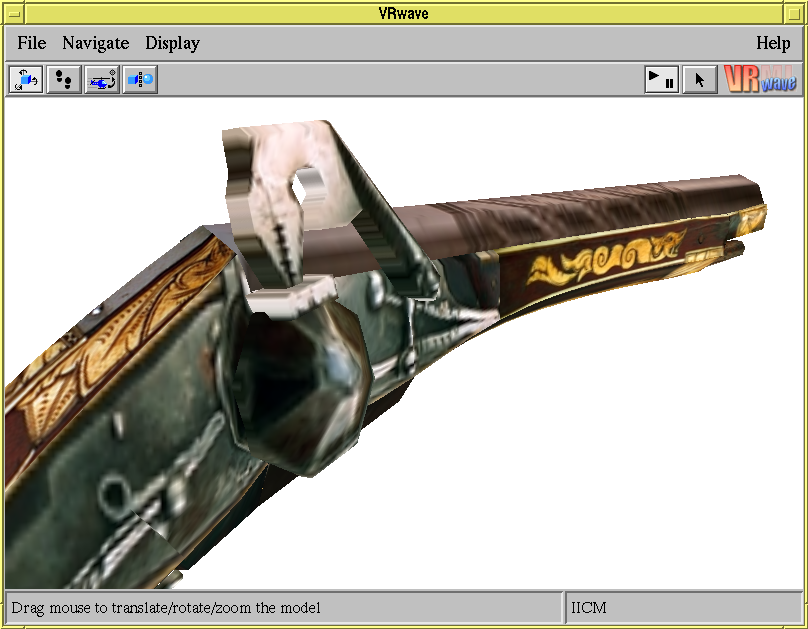
\includegraphics[keepaspectratio,width=\linewidth,height=\halfh]
{images/pist.png}

\caption[VRwave in Flip Mode]
{%
VRwave in Flip mode displaying a textured model of a cavalry pistol
from the world-renowned Zeughaus (armoury) in Graz.
\imgcredit{Image extracted from \textcite[page~81]{Andrews-VRwave}
and used under the terms of the ACM Copyright Policy. \copyrightACM}
}
\label{fig:Pistol}
\end{figure}

The caption shows an example of how to correctly cite the source when
using an image from someone else. In their 1998 paper,
\textcite{Andrews-VRwave} discuss the VRwave VRML browser.




\section{Using Subfigures}

The example in Figure~\ref{fig:RespTable} shows how to use subfigures
within a figure with the \vname{subfig} package. The figure is an
illustration of how a responsive table looks different at different
screen widths. Figure~\ref{fig:RespTableNarrow} shows the table on a
narrow screen, while Figure~\ref{fig:RespTableWide} shows the table on
a wider screen.

The source code shows usage of the \vname{includegraphics} options
\vname{frame} to draw a frame around the graphics and \vname{valign=t}
to top align them, which are both provided by the \vname{adjustbox}
package.  For this figure, it is important to ensure that both images
are scaled equally, hence the use of \vname{scale}. The exact scale
factor was determined by trial and error.


\begin{figure}[tp]
\centering
\subfloat[%  the % chars remove implicit spacing
Narrow screen.
]
{%
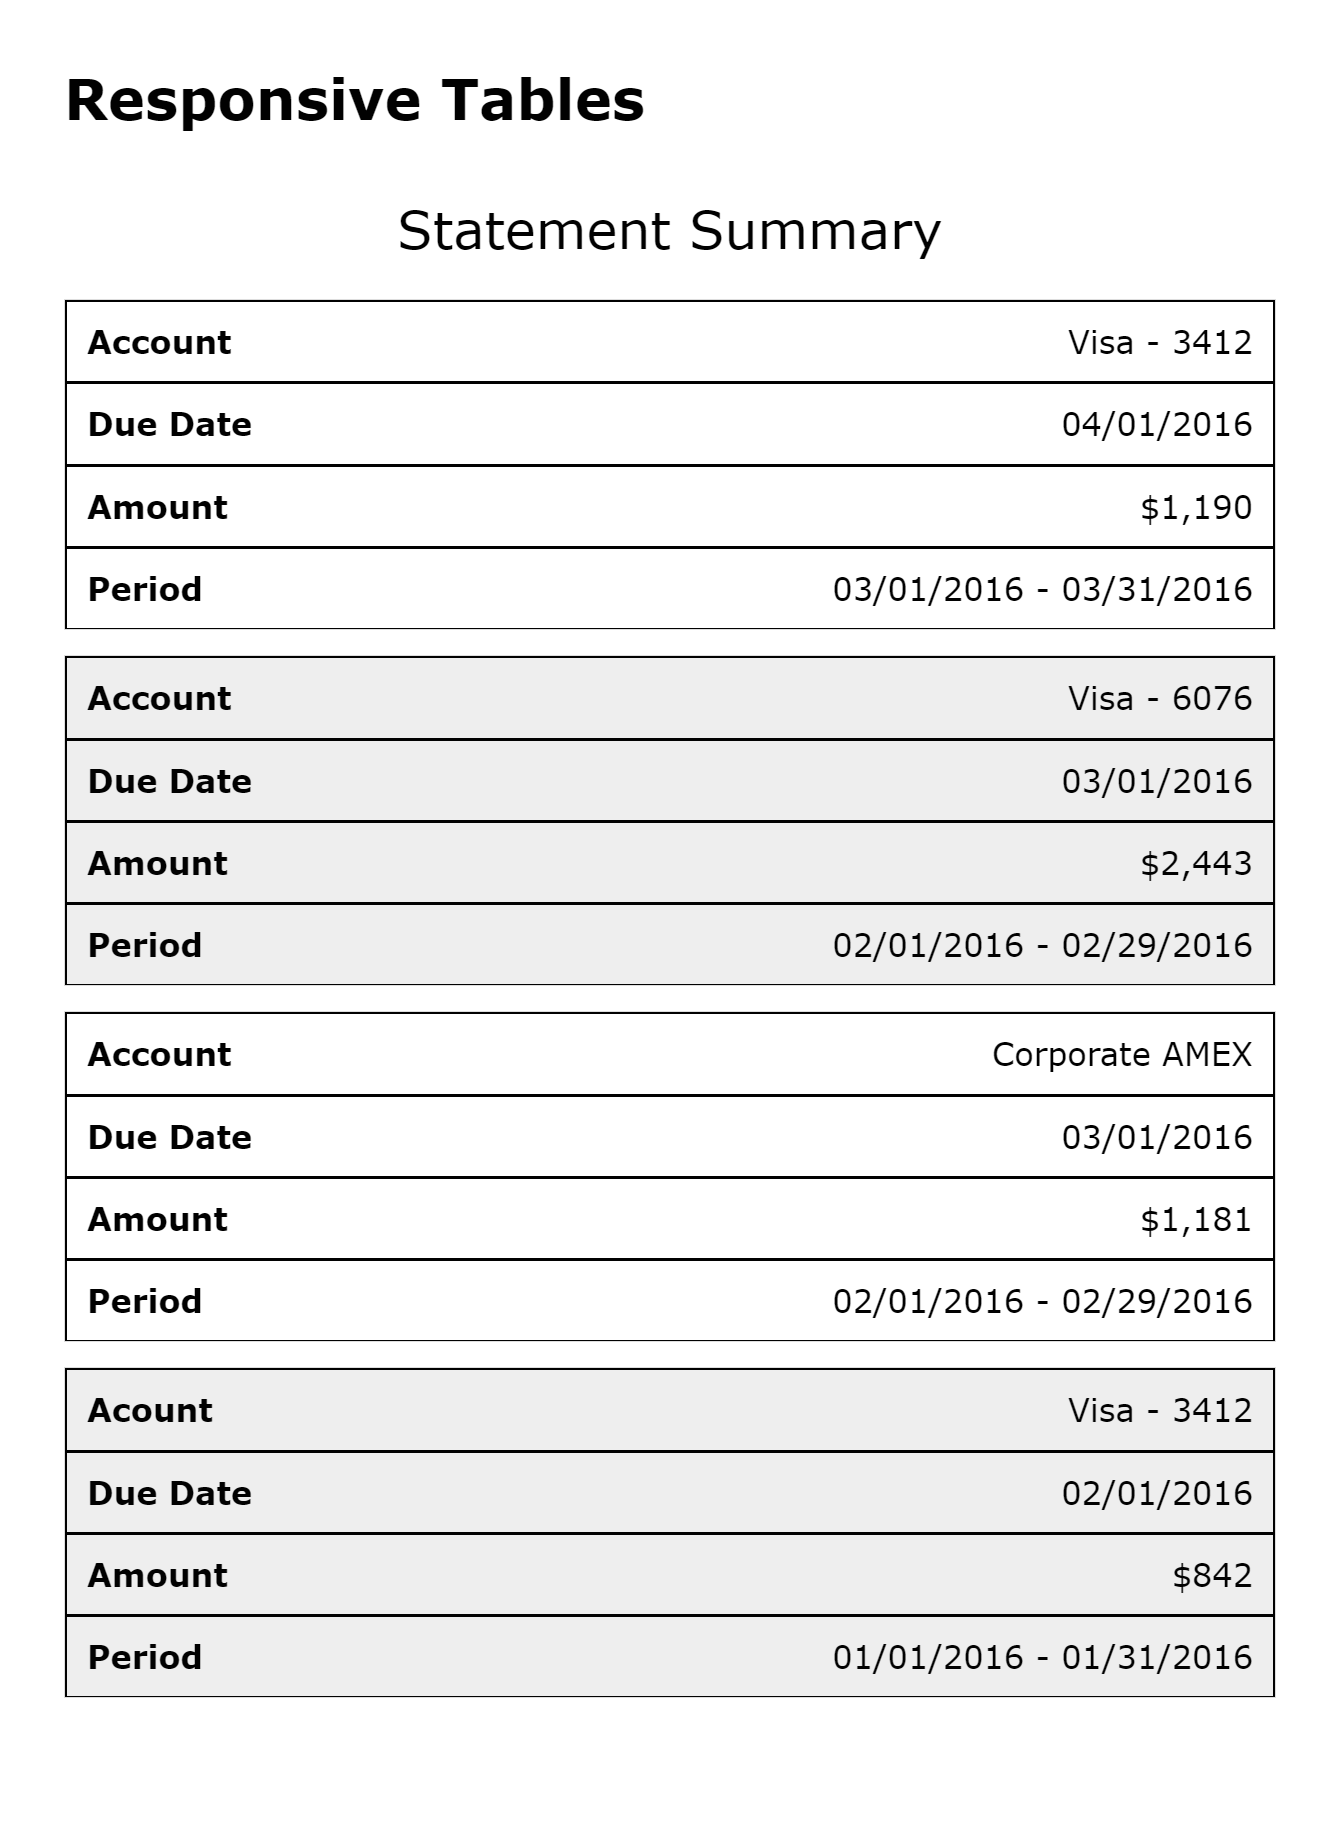
\includegraphics[valign=t,frame,scale=0.32]
{images/rt-2021-11-09-narrow-ci.png}%
\label{fig:RespTableNarrow}%
}
\hfill         % fills up the space between the two graphics
\subfloat[%
Wide ecreen.
]
{%
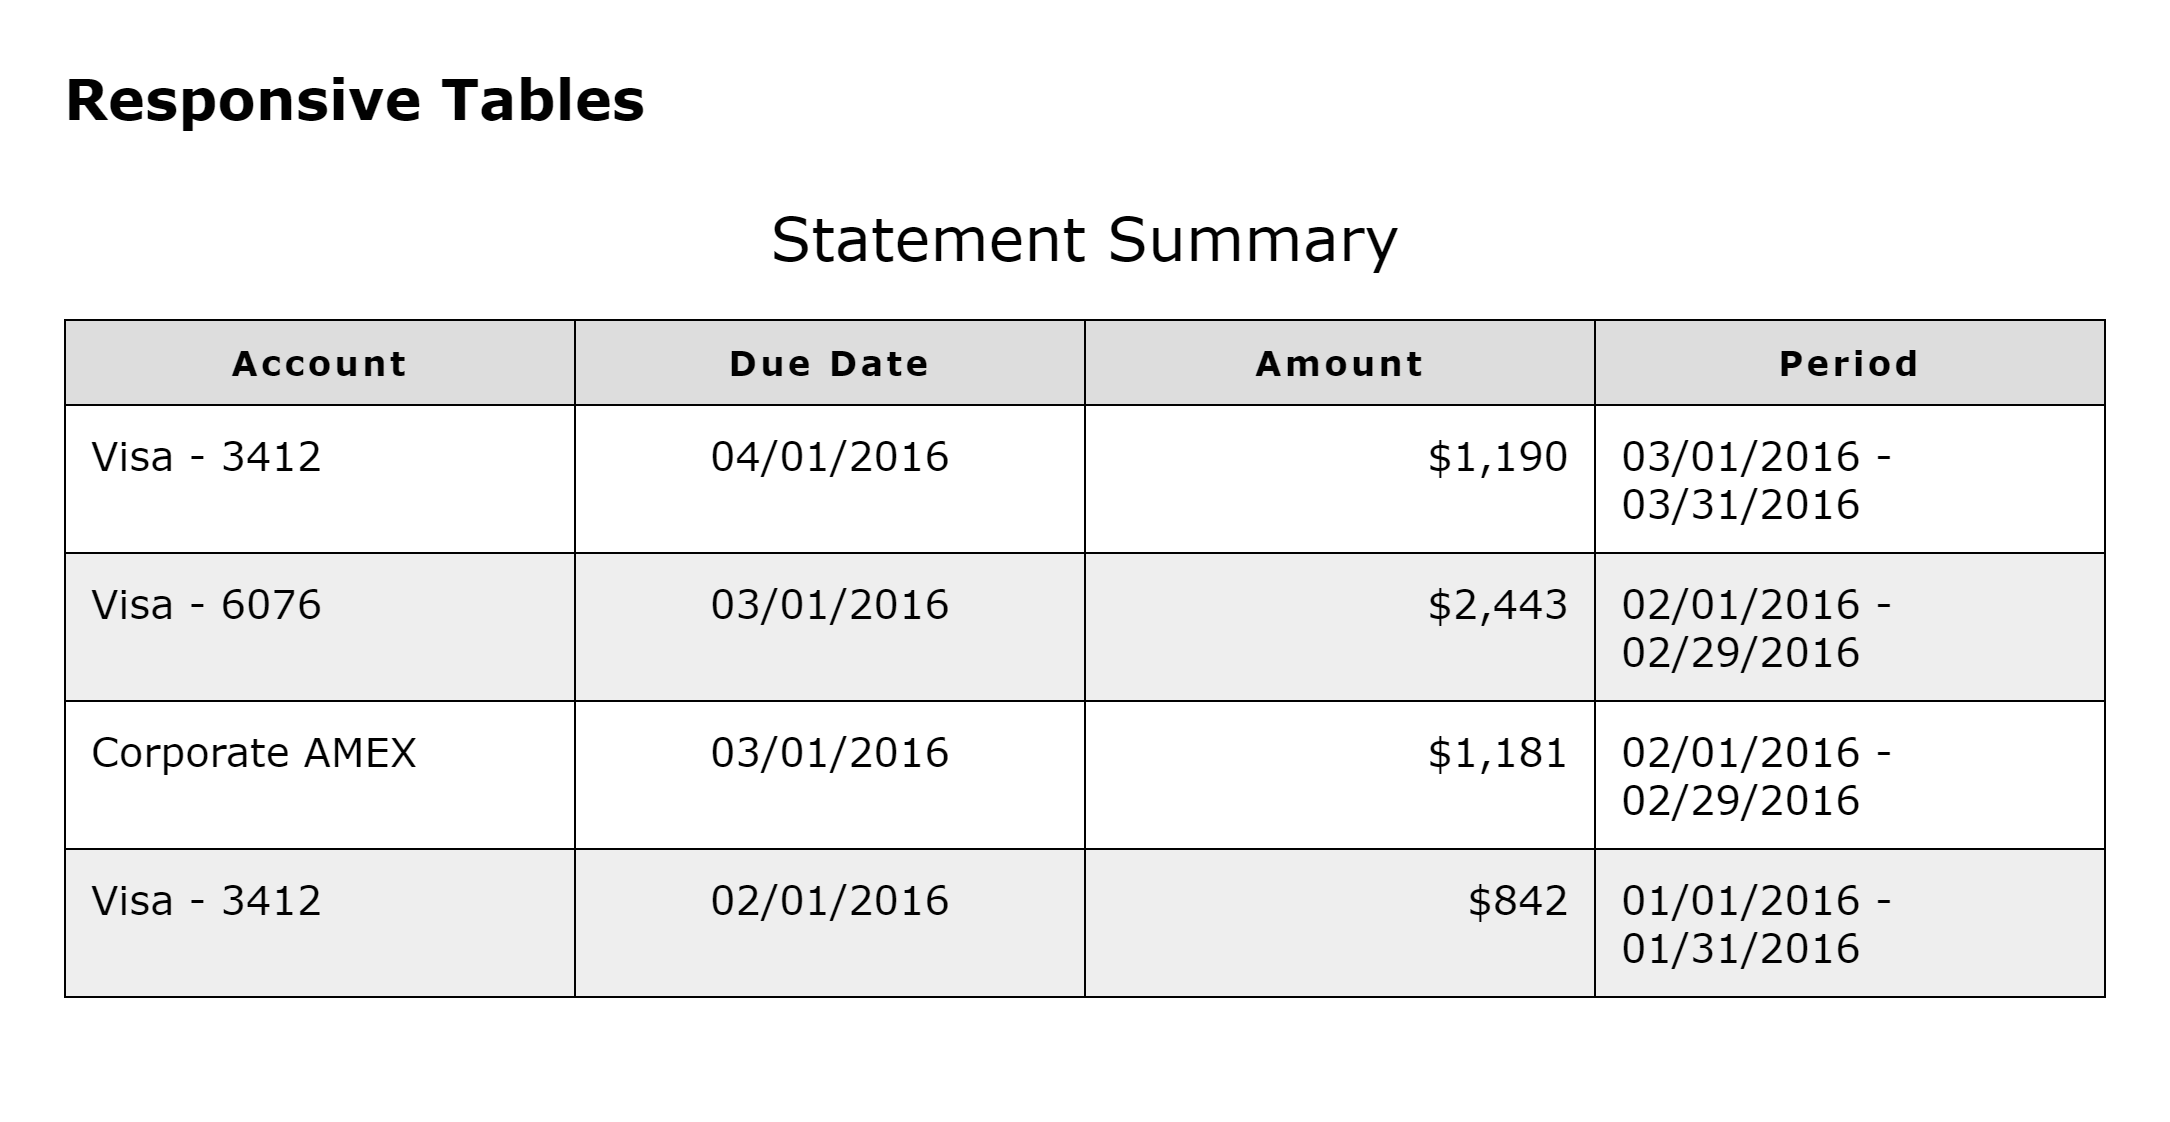
\includegraphics[valign=t,frame,scale=0.32]
{images/rt-2021-11-09-wide-ci.png}%
\label{fig:RespTableWide}%
}

\caption[Responsive Table]
{
A responsive table adapts itself to the available display space. On a
narrow screen, each row of the table is expanded vertically.
\imgcredit{Both images created by Keith Andrews.}
}
\label{fig:RespTable}
\end{figure}







\section{Including Vector Graphics}

Charts and diagrams are often naturally vector graphics, created by
assembling and arranging graphical objects such as lines, boxes,
circles, polygons, and text strings. They can usually be exported or
saved in SVG and then converted to (vector) PDF format, or saved
directly as (vector) PDF. Vector graphics have the huge benefit that
they are freely scalable: they remain crisp and sharp even when zoomed
in.
%
Vector graphics are included in LaTeX as (vector) PDF files, as shown
in Figure~\ref{fig:BreakpointDiagram}. Try zooming in to the figure in
Acrobat Reader.



\begin{figure}[tp]
\centering
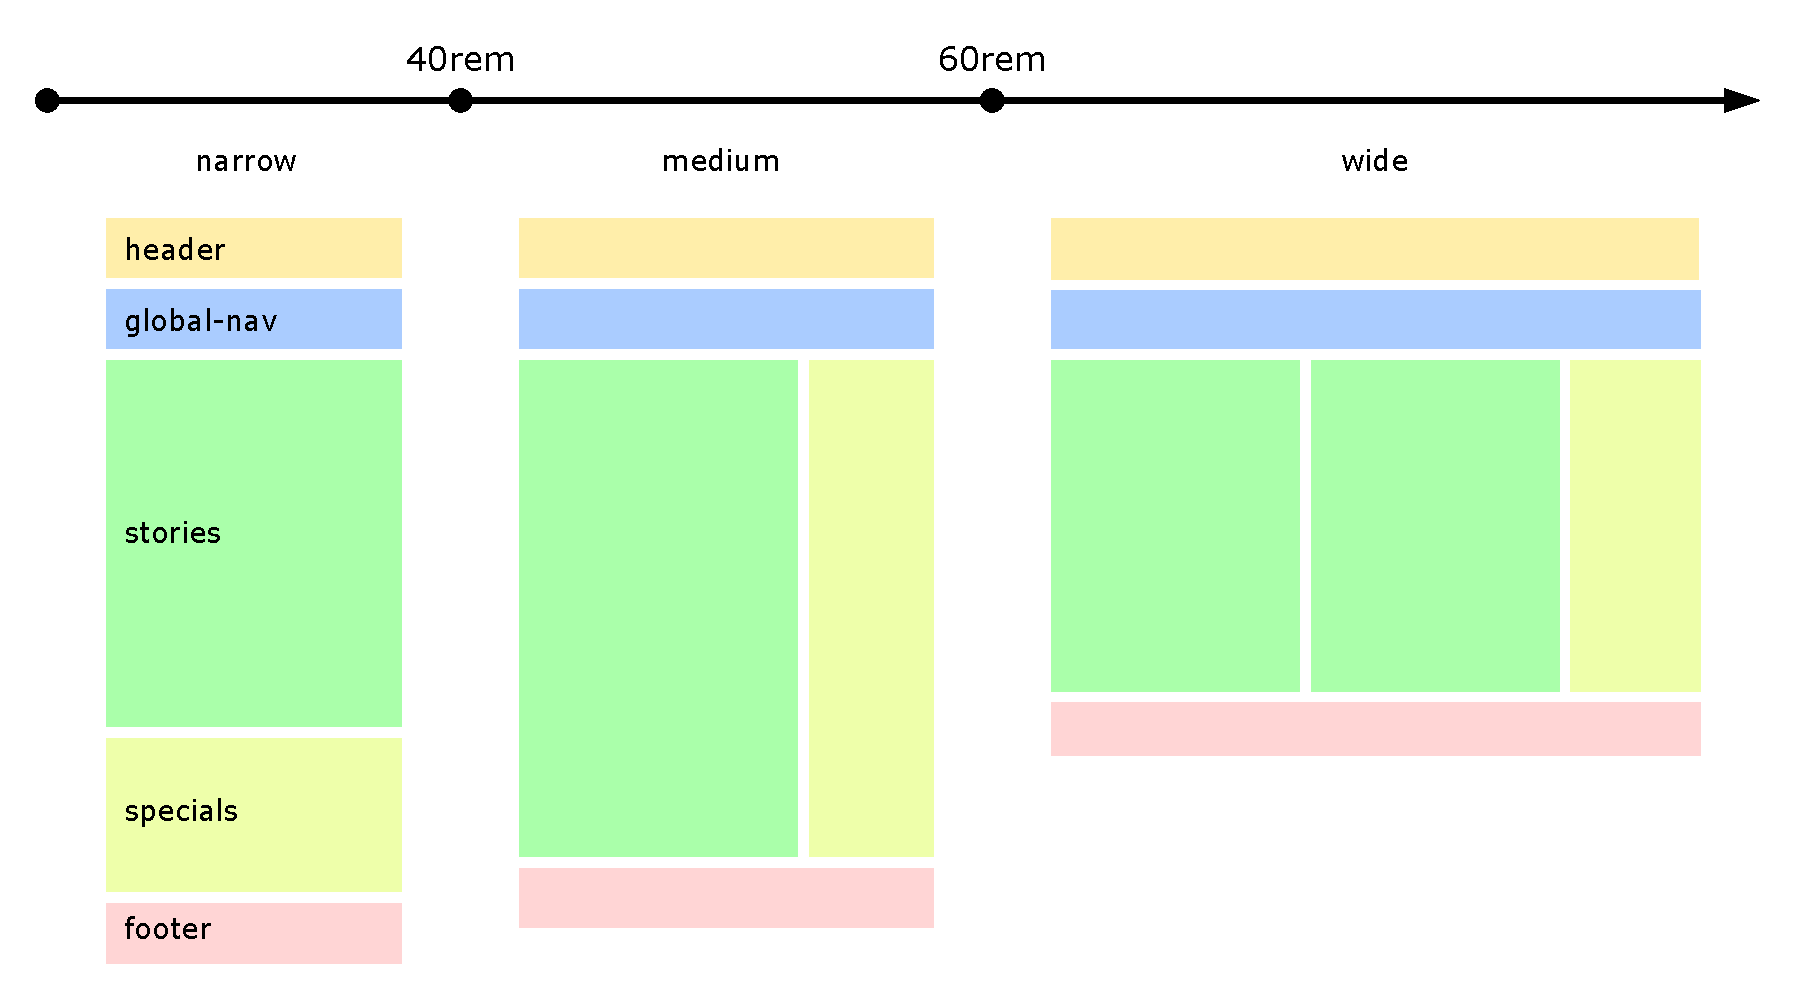
\includegraphics[frame,keepaspectratio,width=\linewidth,height=\halfh]
{diagrams/breakpoint.pdf}

\caption[Responsive Breakpoint Diagram]
{
A responsive breakpoint diagram. Setting breakpoints at 40 rem and 60 rem
provides for three different layouts: narrow, medium, and wide.
The layout scales smoothly between breakpoints and changes at a breakpoint.
\imgcredit{Drawn by Keith Andrews.}
}
\label{fig:BreakpointDiagram}
\end{figure}










\section{Using Tables}

An example of using a table can be seen in Table~\ref{tab:SomePubs}.

\begin{table}[tp]
\tablestretch
\rowcolors{2}{}{tablerowcolour}
\centering
\begin{tabularx}{\linewidth}
{>{\kern-\tabcolsep}lllX<{\kern-\tabcolsep}}
\toprule
\textbf{Name} & \textbf{Type} & \textbf{Rating} & \textbf{Description} \\
\midrule
Flann O'Brien & Irish / International & ***** &
In the centre of town, easy for
marauding tourists to find. Good food, smooth Guinness.\\
%
Dublin Road & Irish & ***** &
In the old town, best Guinness in Graz.
Regular live music. Irish session every Wednesday.\\
%
O'Carolan's & Irish & **** &
In the centre of town in a small side street next to Flann's.
Small, cosy, open late.\\
%
Two Brothers & Irish / English & **** &
Hidden in the narrow streets of the old town.
Erasmus student night on Wednesday.\\
%
O'Sullivan's & Irish / Austrian & **** &
Cosy, friendly place, many regulars.\\
%
O'Riginal & Austrian & ** &
Near to Jakominiplatz.
Small place with Guinness. Regular live music.\\
\bottomrule
\end{tabularx}

\caption[Some Pubs in Graz]
{
Some pubs in Graz.
}
\label{tab:SomePubs}
\end{table}









\section{Using Special Characters and Symbols}

You can use many (but not all) of the thousands of characters
available in the UTF-8 \parencites{Wikipedia-UTF8}{Unicode-Charts}
character encoding. For example, the German umlauts (äüö), the German
sharp s (ß), or the yen symbol (¥).

You can also try some of the \approxsym 100 symbols available
in the \vname{textcomp} package, such as the yen symbol (\textyen) and
a circled letter A (\textcircled{A}).





\section{Using Macros to Style Special Names}

Sometimes, a macro (new command definition) can be useful to style
special names or phrases consistently. For example, if you are often
refering to named components of a user interface, such as the
\uiname{Toolbar} or \uiname{Status Panel}, then define a macro
\verb|uiname|, so that all such components can be styled consitently:
\begin{lstlisting}
\newrobustcmd{\uiname}[1]{{\smaller\textsf{#1}}}
\end{lstlisting}

Macros like \vname{vname}, \vname{cname}, and \vname{fname} can be
used to style (say) variable names, class names, and file names. This
is a long file name
\fname{/usr/data/keith/travel/austria/vienna.txt}. This is a typical
class name in camel case \cname{HVSInformationPyramidsInputFactory}.





\section{Using Floating Listings}

Listing~\ref{list:HTML5Boilerplate} is floating. A floating listing is
a block of code treated like other \LaTeXe floats (such as figures or
tables). Use floating listings for longer blocks of code.
A floating listing is given a number and can be referred to
explicitly, like Listing~\ref{list:HTML5Boilerplate}. It can be given
a caption and short caption, and is listed in the List of Listings.


\begin{samepage}
\begin{lstlisting}[%
  float=tp,
  aboveskip=\floatsep,
  belowskip=\floatsep,
  xleftmargin=0cm,              % no extra margins for floats
  xrightmargin=0cm,             % no extra margins for floats
  language=HTML,
  basicstyle=\footnotesize\ttfamily,
  frame=shadowbox,
  numbers=left,
  label=list:HTML5Boilerplate,
  caption={[HTML5 Boilerplate Code]%
Some HTML5 boilerplate code, illustrating the typical structure
of a HTML5 web page.
},
]
<!DOCTYPE html>
<html xmlns="http://www.w3.org/1999/xhtml" lang="en" xml:lang="en">

<head>
<meta charset="UTF-8"/>
<meta name="viewport" content="width=device-width, initial-scale=1"/>
<link rel="stylesheet" href="./inm.css"/>

<title>Keith Andrews Web Page</title>
</head>

<body>

<header>
<img src="images/kalogo.svg" alt="KA Logo"/>
Keith Andrews Design
</header>

<h1>Keith Andrews</h1>

<p>
Keith lives in <a href="http://graz.at/">Graz</a>.
</p>

<p>
<img src="images/keith-s.jpg"
  alt="Photo of Keith Andrews"/>
</p>

<p>
Three desirable attributes:
</p>
<ol>
<li>cheap</li>
<li>fast</li>
<li>good</li>
</ol>
<p>
Choose any two.
</p>

<p>
<abbr title="Extensible HyperText Markup Language">XHTML</abbr>
is cool.
</p>

<table>
<tbody>
<tr><th>Beer</th><th>Price €</th></tr>
<tr><td>Puntigamer</td><td>2,60</td></tr>
<tr><td>Gösser</td><td>2,60</td></tr>
<tr><td>Guinness</td><td>4,35</td></tr>
</tbody>
</table>

<footer>
Copyright © Keith Andrews 2019.
</footer>

</body>
</html>
\end{lstlisting}
\end{samepage}










\section{Using Non-Floating Diplayed Listings}

The listing below shows some CSS:
\begin{samepage}
\begin{lstlisting}[%
  language=CSS,
]
body { color: black; background-color: silver; }
img { border: none; }
h1,h2 { font-family: Verdana, sans-serif; }
\end{lstlisting}
\end{samepage}
It is displayed (i.e. indented as a block) in-place, but is not
floating. It cannot be referred to by number and is not listed in the
List of Listings. As a rule of thumb, if listings have five or more
lines, make them floating.





\section{Using Inline Listings}

Inline listings are used for very short snippets of code embedded
within the flow of a paragraph. For example,
\lstinline|\lstinline!var i:integer;!|
produces
\lstinline!var i:integer;!, which can now be discussed further.
Do not break an inline listing over multiple lines (EOL).




\section{Using Lists}

A list should always be introduced by a sentence
which ends with a colon.
%
There are three kinds of standard lists in \LaTeXe:
\begin{itemize}
\item itemize
\item enumerate
\item description
\end{itemize}
% A blank line here would indicate a new (indented) paragraph
An enumerated list has numbered items:
\begin{enumerate}
\item Fast
\item Good
\item Cheap
\end{enumerate}
Choose any two!


A description list has named items with corresponding
definitions or descriptions:
\begin{description}
\item[Short] Each item has a label (name) and its description.

\item[Rather longer label] By default, if the description text
  is rather long, it will warp around to the following lines.
\end{description}

